\documentclass[letter,12pt]{article}
\usepackage[letterpaper,right=1.25in,left=1.25in,top=1in,bottom=1in]{geometry}
\usepackage{setspace}

\usepackage[utf8]{inputenc}   % allows input of special characters from keyboard (input encoding)
\usepackage[T1]{fontenc}      % what fonts to use when printing characters       (output encoding)
\usepackage{amsmath}          % facilitates writing math formulas and improves the typographical quality of their output
\usepackage{url}              % adds line breaks to long urls
\usepackage[pdftex]{graphicx} % enhanced support for graphics
\usepackage{tikz}             % Easier syntax to draw pgf files (invokes pgf automatically)
\usetikzlibrary{arrows}

\usepackage{mathptmx}           % set font type to Times
\usepackage[scaled=.90]{helvet} % set font type to Times (Helvetica for some special characters)
\usepackage{courier}            % set font type to Times (Courier for other special characters)

\usepackage[longnamesfirst, sort]{natbib}\bibpunct[]{(}{)}{,}{a}{}{;} % handles biblio and references 

\usepackage{rotating}         % sideway tables and figures that take a full page
\usepackage{caption}          % allows multipage figures and tables with same caption (\ContinuedFloat)

\usepackage[colorlinks=true]{hyperref}

%FOR SPANISH FORMATTING (HYPHENATION ETC.)
\usepackage[spanish]{babel}
\addto\captionsspanish{\renewcommand{\figurename}{Diagrama}} % cambia Figura por Diagrama



\newcommand{\mc}{\multicolumn}

\begin{document}

\textbf{Política Comparada II}

\textbf{Examen parcial}

\textbf{Otoño 2016}

\bigskip

\noindent La gráfica de la página siguiente resume el \emph{UK Polling Report}. Cada punto en el diagrama reporta una encuesta del Reino Unido---o, más precisamente, el porcentaje de intención de voto por un partido (eje vertical) entre los entrevistados de una encuesta. Las fechas de las encuesta (eje horizontal, las unidades son meses con la marca de año centrada en cada enero) van del 13/5/2010 al 2/8/2016. Los colores distinguen los partidos: 
rojo = laboristas; 
azul = conservadores; 
amarillo = liberal-demócratas; 
negro = UKIP; 
verde = partido verde.
(Puede consultar la fuente \href{http://ukpollingreport.co.uk/voting-intention-2}{aquí}.)

\bigskip

\noindent Su trabajo consiste en lo siguiente. 

\begin{enumerate}
\item Identifique en el diagrama un periodo, una tendencia o un patrón interesante. Describa \emph{clara y concisamente} su selección---el lector debe poder entender a qué está refierendo.  
\item Plantee una pregunta.
\item Reporte una historia de 400 palabras relacionada con la selección, que intente dar respuesta a su pregunta, y que diga algo interesante sobre las instituciones británicas y sus partidos. 
\end{enumerate}

\bigskip

Cite el material del curso y las demás fuentes consultadas (aproveche para poner en práctica las recomendaciones de Harvey, en \emph{Writing wth sources}). Indique el total de palabras del apartado 3 (procurando que los 1 y 2 ocupen un puñado de oraciones solamente). El trabajo es individual y deberá entregarlo el 20/9/2016, al iniciar la clase. \textbf{¡Mucha suerte!}

\begin{sidewaysfigure}
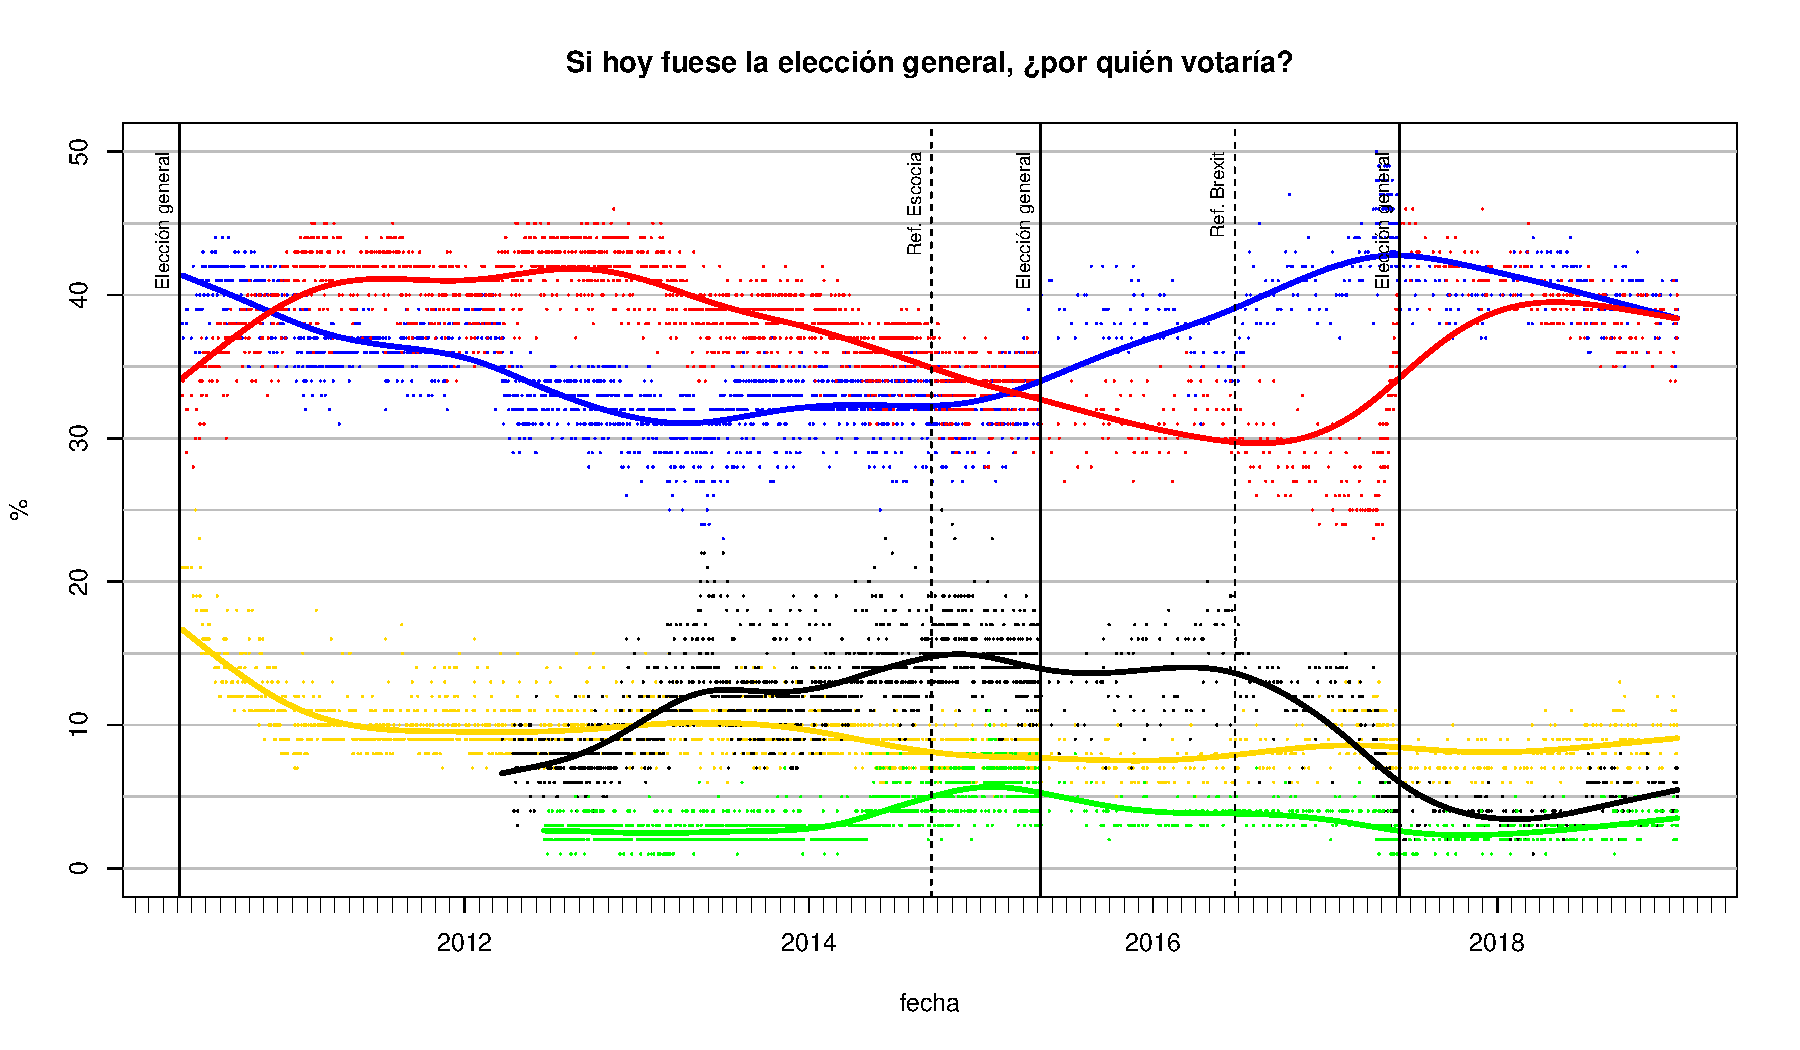
\includegraphics[width=.9\columnwidth]{../data/uk/ukVoteIntentionsSince2010.pdf} \\
\caption{\emph{Poll of Polls} britanico. Preparado por Eric Magar con datos de \protect\url{http://ukpollingreport.co.uk/voting-intention-2}.}
\end{sidewaysfigure}  

\end{document}

